\chapter{Diversidad de fase}
\label{cap:diversidad}

A las técnicas de recuperación de fase no interferométrico pertenece una familia conocida como \textit{Phase Retrieval}; en general, esta familia se basa en algoritmos iterativos para determinar la fase, mediante un problema inverso de múltiples observaciones. El método conocido como diversidad de fase (PD: \textit{phase diversity}) es un tipo de \textit{Phase Retrieval} en donde se añade redundancia al algoritmo de forma que las aberraciones recuperadas son más precisas.\\

%conocido como diversidad de fase (PD: \textit{phase diversity}), el cual  de técnicas de recuperación de fase ; 

%A las técnicas de recuperación de fase no interferométrico pertenece uno conocido como diversidad de fase (PD: \textit{phase diversity}), el cual pertenece a una familia de técnicas de recuperación de fase conocida como \textit{Phase Retrieval}; en general, esta familia se basa en métodos iterativos para determinar la fase.\\

En este capítulo abordaremos el concepto de PD desde su planteamiento inicial para sistemas ópticos con iluminación incoherente y analizaremos el funcionamiento del algoritmo. Analizaremos cómo pueden describirse las aberraciones ópticas a partir de los polinomios de Zernike, y luego plantearemos un nuevo PD para sistemas con iluminación coherente. Posteriormente se propondrán dos modificaciones sobre PD coherente basadas en la curva de modulación en fase del SLM. En la sección \ref{sec:est_arte} se hará una breve introducción sobre PD. A continuación en la sección \ref{sec:div_fase_trad} se abordará el concepto de PD. En la sección \ref{sec:aberraciones} se tratarán las aberraciones ópticas a partir de los polinomios de Zernike; luego en la sección \ref{sec:PD_coherente} se planteará un modelo de PD para sistemas con iluminación coherente, lo cual es una ampliación del Capítulo \ref{cap:vortices}. Finalmente, en la sección \ref{sec:pd12} plantearemos dos modificaciones sobre PD coherente que permitirán diferenciar las aberraciones que son ocasionadas por la modulación de un SLM con las del sistema óptico.

%Dado que el método implementado para la detección de las aberraciones presentes en vórtices ópticos surge de una técnica empleada en sistemas con iluminación incoherente conocida como diversidad de fase (PD: \textit{phase diversity}), en este capítulo analizaremos a fondo la propuesta tradicional de PD y las modificaciones realizadas sobre este, a fin de obtener no solo un PD coherente, si no que a partir de este generar dos conceptos de corrección adicionales basados en información adicional del SLM. Con estos nuevos conceptos se pretende poder distinguir la contribución a las aberraciones del sistema óptico y del SLM. A continuación, la sección \ref{sec:est_arte} es una revisión histórica del desarrollo de PD. En la sección \ref{sec:div_fase_trad} se presentará el postulado inicial de PD, es decir, desde la reconstrucción en sistemas con iluminación incoherente. En la sección \ref{sec:aberraciones} veremos por qué es posible expresar un frente de onda en términos de una serie de los bien conocidos polinomios de Zernike y cómo se puede aplicar esto a PD. Luego, retomaremos PD para proponer su aplicación a sistemas con iluminación coherente y en específico a OVs en la sección \ref{sec:PD_coherente}. Finalmente, veremos cómo a partir de información adicional del SLM y de PD coherente podemos plantear un modelo de determinación de aberraciones causadas por sistemas ópticos y por SLMs.

%Diversidad de fase (PD: \textit{phase diversity}) es un método no interferométrico de sensado de fase que pertenece a una familia de métodos de recuperación de fase conocida como \textit{Phase Retrieval}, en general, esta familia se basa en la determinación de la fase de una manera iterativa.\\

%En este capítulo abordaremos el concepto de PD desde su planteamiento inicial para sistemas ópticos con iluminación incoherente y analizaremos cómo funciona en este caso el algoritmo. Analizaremos cómo pueden describirse las aberraciones ópticas a partir de los polinomios de Zernike, y luego plantear un nuevo PD para sistemas con iluminación coherente y posteriormente se propondrán dos modificaciones sobre PD coherente. En la sección \ref{sec:est_arte} se hará una breve introducción sobre PD. A continuación en la sección \ref{sec:div_fase_trad} se abordará el concepto de PD. En la sección \ref{sec:aberraciones} se tratarán las aberraciones ópticas a partir de los polinomios de Zernike, luego en la sección \ref{sec:PD_coherente} se planteará un modelo de PD para sistemas con iluminación coherente, lo cual es una ampliación del Capítulo \ref{cap:vortices}. Finalmente, en la sección \ref{sec:pd12} plantearemos dos modificaciones sobre PD coherente que permitirán diferenciar las aberraciones que son ocasionadas por la modulación de un SLM con las del sistema óptico.


\section{Introducción}
\label{sec:est_arte}

%(PD: \textit{Phase diversity})

El método de PD fue planteado en 1982 por Gonsalves \cite{Gonsalves1982}, quien propone un sensor de frente de onda (WFS: \textit{Wave-front sensor}) basado en la captura de dos imágenes simultáneas de una misma fuente, en donde una de las imágenes se encuentra en un plano focal, mientras que la otra se encuentra desenfocada una cantidad conocida. A la imagen adicional que se encuentra desenfocada, se le conoce como \textit{diversidad de fase}. En este caso, Gonsalves parametriza la fase en términos de los polinomios de Zernike y demuestra por medio de simulaciones, que a través de un algoritmo iterativo puede obtenerse una estimación de las aberraciones del sistema óptico. \\

En 1988 Paxman et al \cite{Paxman1988} emplean la técnica planteada por  Gonsalves para sensar desalineamientos en telescopios de múltiples espejos deformables. Allí, además de corregir el desalineamiento, logran compensar las aberraciones que se introducen debido a la turbulencia atmosférica, resultado simulado anteriormente por Gonsalves. Pero es en 1992 cuando Paxman et al \cite{Paxman1992} proponen emplear PD como sensor de aberraciones para sistemas ópticos con iluminación incoherente, considerando un número arbitrario de diversidades de fase.% Desde entonces PD ha sido empleado en diferentes problemas que involucran óptica adaptativa \cite{Lofdahl1994, Korkiakoski2012, Sauvage2007, Schgallis2007} o como WFS \cite{Bonet2005, Sauvage2012, Lofdahl1998}, por ejemplo, Lofdahl1994 et al \cite{Lofdahl1994} lo emplean para la corrección de frentes de onda mediante el control de espejos de espejos deformables.

%Pero es en 1992 cuando Paxman et al \cite{Paxman1992} proponen emplear PD como sensor de aberraciones para sistemas ópticos con iluminación incoherente, considerando un número arbitrario de diversidades de fase. Desde entonces PD ha sido empleado en diferentes problemas que involucran óptica adaptativa, observación solar o WFSs \cite{Lofdahl1994, Bonet2005, Korkiakoski2012, Sauvage2007, Sauvage2012, Lofdahl1998, Schgallis2007}.

\section{Diversidad de fase incoherente}
\label{sec:div_fase_trad}

%Como se mencionó anteriormente, PD es un método de sensado de frente de onda para sistemas ópticos con iluminación incoherente, que al igual que otros métodos no interferométricos se basa en medidas de intensidad del campo que se propaga por un sistema óptico. En este se emplean dos imágenes, una que proviene de un plano focal y otra que proviene de un plano desenfocado una distancia conocida $d$, como se muestra en la Fig. \ref{fig:pd}. 
%Este método es no interferométrico y por la, cuando se recupera solo la aberración del sistema óptico corresponde a PD, pero cuando se hace una estimación del objeto y la fase se refiere a PR.\\

Como se mencionó anteriormente, PD es un método de sensado de frente de onda que pertenece a una categoría de WFSs no interferométricos conocidos como \textit{Phase Retrieval}, estos se basan en medidas de intensidad para recuperar de manera iterativa las aberraciones causadas por un sistema óptico empleando o bien esquemas de propagación o algoritmos de búsqueda de gradiente (GSAs: \textit{gradient search algorithm}). PD está planteado para ser un algoritmo de tipo GSA, de modo que a través de un problema inverso de múltiples observaciones se recupera la fase. En su planteamiento inicial se emplean dos imágenes, una que proviene de un plano focal y otra que proviene de un plano desenfocado una distancia conocida $d$, como se muestra en la Fig. \ref{fig:pd}. \\


\begin{figure}[!ht]
  \centering
    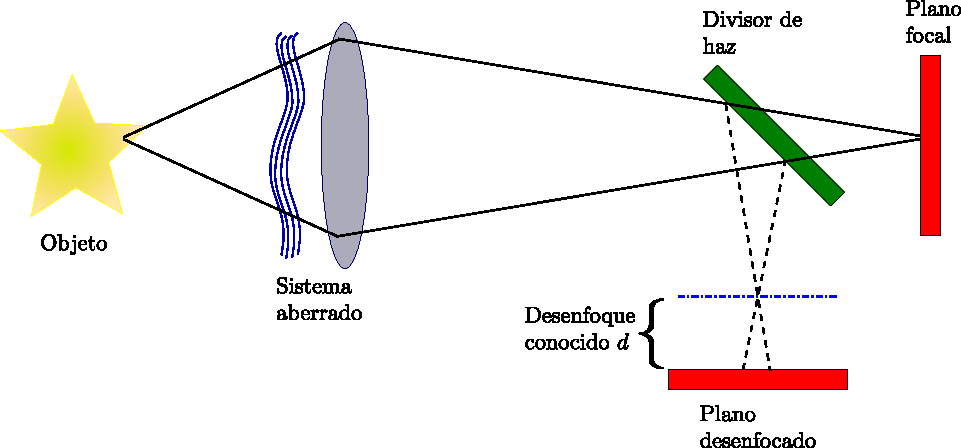
\includegraphics[width=\textwidth,keepaspectratio]{Caps/Imagenes/pd.pdf}
  \caption{Esquema de PD incoherente.}
  \label{fig:pd}
\end{figure}

Consideremos un objeto que es iluminado con luz espacialmente incoherente, si el sistema es lineal\footnote{Recordemos que los sistemas ópticos con iluminación incoherente son lineales con respecto al módulo cuadrado de la amplitud compleja, es decir, con respecto a la intensidad.} e invariante ante el desplazamiento, el plano imagen $d(\vec{x})$ que produce dicho objeto es,

\begin{equation}
\label{eqD1}
	d(\vec{x})= d_{obj}(\vec{x}) \otimes s(\vec{x}),
\end{equation}

donde $\vec{x}$ es un vector de posición bidimensional de coordenadas $(x,y)$, $s(\vec{x})$ la función de punto extendido (PSF: \textit{point-spread function}), $d_{obj}(\vec{x})$ es la irradiancia ideal de la imagen obtenida desde la óptica geométrica \cite{Goodman2005} y $\otimes$ representa la función convolución definida como,
%%% 
%d_obj esta definida como desde el plano imagen se vería el objeto usando la óptica geométrica sin aberraciones
%%%
\begin{equation}
\label{eqD1a}
\begin{aligned}
	d_{obj}(x,y) \otimes s(x,y) & = \mathscr{F}^{-1}\{ \mathscr{F}\{d_{obj}(x,y)\} \mathscr{F} \{s(x,y)\}\}\\
	& = \iint\limits_{-\infty}^{\infty} d_{obj}(\xi,\eta) s(x-\xi,y-\eta) d\xi d\eta
\end{aligned}
\end{equation}

De acuerdo al teorema de la convolución podemos expresar la Eq. \ref{eqD1} en función de sus transformadas de Fourier (FTs: \textit{Fourier transforms}),

%donde $\vec{x}$ es un vector de posición, $d_{obj}(\vec{x})$ el plano objeto, $s(\vec{x})$ la función de punto extendido (PSF: \textit{point-spread function}) y $\otimes$ representa la función convolución definida como. De acuerdo al teorema de la convolución podemos expresar la Eq. \ref{eqD1} en función de sus transformadas de Fourier así

\begin{equation}
\label{eqD2}
	D(\vec{u}) = D_{obj}(\vec{u}) S(\vec{u}),
\end{equation}

donde $\vec{u}$ es un vector de frecuencias espaciales bidimensionales definido en términos de $(\xi , \eta)$, $D(\vec{u}) = \mathscr{F}\{d(\vec{x})\}$, $D_{obj}(\vec{u}) = \mathscr{F} \{d_{obj}(\vec{x})\}$ y $S(\vec{u})=\mathscr{F} \{s(\vec{x})\}$. Para un sistemas con iluminación incoherente $S(\vec{u})$ es la función de transferencia óptica (OTF: \textit{optical transfer function}) \cite{Goodman2005} y puede definirse como,

\begin{equation}
\label{eqD3}
	S(\vec{u}) = H(\vec{u}) \star H(\vec{u}),
\end{equation}

que es la autocorrelación de la función de transferencia coherente $H(\vec{u})$ (CTF: \textit{coherent transfer function}) dada por,

\begin{equation}
\begin{aligned}
	H(\xi,\eta) \star H(\xi,\eta) &= H(\xi,\eta) \otimes H^{\ast}(-\xi,-\eta) 
	\\&= \iint\limits_{-\infty}^{\infty} H(p,q) H^{\ast}(p-\xi,q-\eta) dp dq.
	\end{aligned}
\end{equation}

La FT de la función de respuesta al impulso $h(\vec{x})$ corresponde a $H(\vec{u})$, y $h(\vec{x})$ está relacionada con la PSF, dado que $s(\vec{x}) = |h(\vec{x})|^2$, es decir, la función pupila generalizada (GP: \textit{generalized pupil}), y tiene la forma,

%Sabemos que $H(\vec{u})$ es la FT de la función de respuesta al impulso $h(\vec{x})$ y que $h(\vec{x})$ está relacionada con la PSF, ya que $|h(\vec{x})|^2$ es la PSF, es decir, la función pupila generalizada (GP: \textit{generalized pupil}) y tiene la forma,

%A su vez, la CTF en la Eq. \ref{eqD3} tiene la forma

\begin{equation}
\label{eqD4}
	H(\vec{u}) = \mathscr{F}\{h(\vec{x})\} = A(\vec{u}) \exp\{i \phi(\vec{u})\},
\end{equation}

con $A(\vec{u})$ definida como la tramitancia de la pupila y $\phi(\vec{u})$ la fase introducida por la pupila en el plano de Fourier si estamos en un sistema $4f$, como es nuestro caso.\\ %es decir, $H(\vec{u})$ puede interpretarse como la función pupila generalizada. Como es bien sabido, a través de función pupila generalizada se pueden describir las contribuciones de fase introducidas por el sistema óptico en un plano de Fourier así como la forma y tramitancia de la apertura.

Si modificamos la GP, por ejemplo, añadiendo una diversidad de fase conocida de forma $\Delta H_1 = \exp(\Delta \phi_1 (\vec{u}))$, tenemos una nueva GP $H_1(\vec{u})$ tal que,

\begin{equation}
\label{eqD4a}
\begin{aligned}
	H_1(\vec{u}) & = A(\vec{u}) \exp\{i [ \phi(\vec{u}) + \Delta \phi_1(\vec{u})] \}\\
	& = H(\vec{u}) \Delta H_1(\vec{u}).
\end{aligned}
\end{equation}

De forma que si tomamos la autocorrelación de esta nueva GP ($S_1(\vec{u})$), produciremos una versión distorsionada $D_1(\vec{u})$ de la imagen inicial $D(\vec{u})$, dado que,

\begin{equation}
	D_1(\vec{u}) = D_{obj}(\vec{u}) H_1(\vec{u}),
\end{equation}

la diferencia entre $D(\vec{u})$ y $D_1(\vec{u})$ está dada justamente por la diversidad de fase que hemos añadido. Si podemos agregar un conjunto de $j$ diversidades de fase a la GP, entonces produciremos $D_{j}(\vec{u})$ imágenes distorsionadas, con $j=1,2,...,k$, de $D(\vec{u})$, y para estas tenemos que,


%por tanto la diferencia entre $G(\vec{u})$ y $G_1(\vec{u})$ es la diversidad de fase que hemos añadido. En PD se encuentran las aberraciones a través de la búsqueda de una distribución de fase $\phi (\vec{u})$ que junto con la tramitancia de la pupila $A (\vec{u})$ recupere la OTF que produce no solo la imagen inicial $G(\vec{u})$, si no que además produce la imagen distorsionada $G_{1}(\vec{u})$. Si podemos agregar un conjunto de $k$ diversidades de fase a la pupila generalizada, entonces produciremos $G_{1...k}(\vec{u})$ imágenes distorsionadas de $G(\vec{u})$ y para estas se tiene que,

%El objetivo de encontrar las aberraciones de fase en PD consiste en buscar una distribución de fase $\phi (\vec{u})$ que junto con la tramitancia de la pupila $A (\vec{u})$ recupere la OTF que produce no solo la imagen inicial $G(\vec{u})$, si no que además produce la imagen distorsionada $G_{1}$. Si podemos agregar $k$ diversidades de fase a la pupila generalizada, entonces produciremos $G_{1...k}$ imágenes distorsionadas y para estas se tiene que,

%Ahora de acuerdo al concepto de PD hay un conjunto de $k$ imágenes (que pueden ser dos o más) en las cuales el objeto se mantiene constante y hay una diversidad de fase, a partir de las expresiones \ref{eqD2} - \ref{eqD4a} para las $k$ imágenes se tiene que

\begin{equation}
\label{eqD7}
	D_j(\vec{u}) = D_{obj}(\vec{u}) S_j (\vec{u}),
\end{equation}

donde,

\begin{equation}
\label{eqD6}
	S_j(\vec{u}) = H_j(\vec{u}) \star H_j(\vec{u}),
\end{equation}

\begin{equation}
\label{eqD5}
	H_j(\vec{u}) = H(\vec{u})\Delta H_j(\vec{u}).
\end{equation}

%(diferencia que está dada o bien por la variación de fase conocida o por superposición de la variación de fase conocida con las aberraciones que agregue el sistema). \\

Esto quiere decir que cada una de las $j$ diversidades si bien poseen la misma información del objeto, su función de transferencia puede ser diferente puesto que hemos añadido una fase adicional conocida. El objetivo de PD es entonces, encontrar una distribución de fase $\phi (\vec{u})$ que junto con la tramitancia de la pupila $A (\vec{u})$ recupere la OTF que produce no solo la imagen inicial $D(\vec{u})$, sino que además produce las imágenes distorsionadas $D_{j}(\vec{u})$.\\

De la Eq. \ref{eqD7} podemos ver que

\begin{equation}
\label{eqD8}
	D_j(\vec{u}) - D_{obj}(\vec{u}) S_j(\vec{u}) = 0,
\end{equation}

es decir, la Eq. \ref{eqD8} es una medida del error entre la imagen obtenida $D_j(\vec{u})$ y la producida idealmente desde la óptica geométrica $D_{obj}(\vec{u})$ modulada por la PSF. Aquellas implementaciones que se basan en GSA \cite{Paxman1992, Echeverri2015} emplean métodos de búsqueda de gradiente, para optimizar funcionales de la forma,

\begin{equation}
\label{eqD8a}
L(\overline{D}_{obj}, \phi) = \sum\limits_{j=0}^K \sum\limits_{m,n}^{M,N} |D_j(m,n) - \overline{D}_{obj}(m,n) S_j(m,n,\phi)|^2,
\end{equation}

donde $\overline{D}_{obj}$ es la FT del objeto recuperado por el sistema óptico hasta la frecuencia de corte y $D_j$ es la FT de la intensidad medida en cada pixel $(m,n)$ luego de añadir una diversidad de fase conocida $j$. En la práctica el objeto real $D_{obj}$ es desconocido y el funcional de la Eq. \ref{eqD8a} se puede expresar en términos de la fase $\phi$ exclusivamente \cite{Paxman1992, Gonsalves1982}.\\


%Emplear optimización no lineal permiten estimar el objeto y las aberraciones de manera conjunta
%Si tomamos el error cuadrático medio para cada punto en la medida brindada por Eq. \ref{eqD8}, tenemos que el error $E$ es,

%\begin{equation}
%\label{eqD9}
%	E = \sum\limits_{j=0}^{K} \sum\limits_{u,v}^{M,N} |G_j(\vec{u}) - D_{obj}(\vec{u}) S_j(\vec{u})|^2,
%\end{equation}
%
%
%
%donde $D_{obj}(\vec{u})$ es la transformada de Fourier del objeto restaurado por el sistema óptico y $G_{k}(\vec{u})$ es la transformada de Fourier de la intensidad medida luego de agregar una aberración conocida de índice $k$, y el error es entonces, la diferencia para cada punto $\vec{u}$ entre el objeto y la imagen para cada diversidad $k$. Eventualmente Eq. \ref{eqD9} es una estimación de la diferencia punto a punto ($\Sigma_u$) de la transformada de Fourier de la imagen obtenida y la transformada de Fourier del objeto restaurado para cada una de las diversidades de fase ($\Sigma_j$). El objetivo es entonces a través de un método iterativo basado en búsqueda del gradiente (GSA: \textit{gradient search algorithm}) encontrar una PSF tal que el error $E$ sea un valor mínimo, de manera que la fase $\phi (\vec{u})$ obtenida sea la que corresponde a la fase inducida por el sistema óptico.

%al aplicar una corrección sobre la pupila del sistema puedan corregirse las aberraciones.\\


%Esta corrección normalmente se hace de manera computacional, de forma que a través de posprocesamiento se pueda recuperar la información del objeto. Ahora bien, de $H_j(\vec{u})$ es fácil obtener la amplitud de la función pupila generalizada, que normalmente es una máscara binaria constante y el problema se reduce a encontrar una fase $\phi_j(\vec{u})$ que es la información de las aberraciones presentes durante la propagación. Esto es lo que se busca con el algoritmo de PD, aunque si no se conoce el objeto \textit{a priori}, la estimación también debe hacerse sobre este \cite{Paxman1992}.\\

%Debido a que nuestro objetivo es encontrar un conjunto de aberraciones parametrizadas que describan la fase de un sistema formador de imagen, basado en la siguiente sección trataremos las aberraciones ópticas.\\
Puesto que uno de nuestros objetivos es poder recuperar aberraciones en un sistema formador de imagen, en la siguiente sección trataremos las aberraciones ópticas

\section{Aberraciones ópticas}
\label{sec:aberraciones}

Las aberraciones pueden ser entendidas como la diferencia de camino acumulado por una superficie Gaussiana de referencia \cite{Goodman2005} (frente de onda esférico perfecto producido por la pupila de salida del sistema y que converge hacia un punto imagen ideal) y el frente de onda real, como se muestra en la Fig. \ref{fig:wf}. Normalmente han sido descritas en términos de los polinomios de Zernike, que son una base ortogonal y completa. Además, han sido aceptados por la Socidad de Óptica (OSA: \textit{Optical Solciety}) como medio de descripción de aberraciones ópticas en sistemas formadores de imagen, aunque no es la única base en la que puedan ser descritas \cite{Schmidt2010, Dai2008}.\\

%Las aberraciones pueden ser entendidas como la diferencia de camino acumulado por una superficie Gaussiana de referencia \cite{Goodman2005} (frente de onda esférico perfecto producido por la pupila de salida del sistema y que converge hacia un punto imagen ideal) y el frente de onda real, como se muestra en la Fig. \ref{fig:wf}. Normalmente han sido descritas en términos de los polinomios de Zernike, que son una base ortogonal y completa. Además, han sido aceptados por la Socidad Americana de Óptica (OSA: \textit{Optical Solciety of America}) como medio de descripción de aberraciones ópticas en sistemas formadores de imagen, aunque no es la única base en la que puedan ser descritas \cite{Schmidt2010, Dai2008}.

\begin{figure}[!ht]
  \centering
    \includegraphics[scale=1]{Caps/Imagenes/wf.pdf}
  \caption[Función aberración definida a partir de una esfera Gaussiana ideal.]{Función aberración definida a partir de una esfera Gaussiana ideal, $W(x,y)$ corresponde al frente de onda aberrado.}
  \label{fig:wf}
\end{figure}

Los polinomios de Zernike están definidos como \cite{Schmidt2010},

\begin{equation}
\label{eqD10}
	Z^{m}_{n}(r,\theta) = \sqrt{2(n+1)}R^{m}_{n}(r)G^{m}(\theta),
\end{equation}

donde $(r,\theta)$ denota coordenadas esféricas, $n$ y $m$ son índices de variación radial y frecuencia azimutal respectivamente, $R(r)$ es una función radial y $G(\theta)$ es una función azimutal. Existe otra forma de escribir los coeficiente $n$ y $m$ bajo un índice único $i$, dado por,

\begin{equation}
\label{eqD11}
	i = \frac{n^2+2n+m}{2},
\end{equation}

de manera que Eq. \ref{eqD10} adquiere la forma,

\begin{equation}
	Z_i (r,\theta) = \left\{
	\begin{array}{l l}
		\sqrt{2(n+1)}R^{m}_{n}(r)G^{m}(\theta) & \quad \text{si $m\neq 0$} \\
		R^{0}_n(r) & \quad \text{si $m = 0$}
	\end{array} \right.
\end{equation}

Las funciones $R(r)$ y $G(\theta)$ están dadas por,

\begin{equation}
\label{eqD12}
	R^m_n(r) = \sum^{(n-m)/2}_{k=0} \frac{(-1)^k(n-k)!r^{n-2k}}{k!(\frac{n+m}{2}-k)!(\frac{m-n}{2}-k)!},
\end{equation}

\begin{equation}
\label{eqD13}
	G^m(\theta) = \left\{
	\begin{array}{l l}
		\cos(m\theta) & \quad \text{si $i$ es par}\\
		\sin(m\theta) & \quad \text{si $i$ es impar}
	\end{array} \right.
\end{equation}

Por último, para que los polinomios de Zernike sean ortogonales, éstos deben estar definidos sobre un círculo unitario \cite{Dai2008}, por tanto,

\begin{equation}
\label{eqD14}
	|r| \leq 1 \quad \forall \quad Z_i(r,\theta).
\end{equation}

\subsection{Ortogonalidad y composición de los polinomios de Zernike}
\label{subsec:ortogonalidad}


Podemos encontrar que los polinomios de Zernike son ortognales desarrollando las expresiones \ref{eqD11} - \ref{eqD14} en la Eq. \ref{eqD10}, de forma que,

\begin{equation}
\label{eqD15}
	\int_{0}^{1} R^{m}_n(\rho) R^m_{n'}(\rho) r dr = \frac{1}{2n+1} \delta_{nn'},
\end{equation}

\begin{equation}
\label{eqD16}
	\int_0^{2\pi}G^m(\theta)G^{m'}(\theta) d\theta= \pi \delta_{mm'},
\end{equation}

\begin{equation}
\label{eqD17}
	\int_0^{2\pi} \int_0^1 Z_n^m (\rho,\theta) Z_{n'}^{m'} (\rho, \theta) rdrd\theta = \pi \delta_{nn'} \delta_{mm'} = \pi \delta_{ii'}
\end{equation}

donde $\rho = r/r_{max}$ es decir, la posición radial normalizada y $\delta_{ii'}$ es el delta de Kronecker que está definido como,

\begin{equation}
\label{eqD18}
	\delta_{ii'} = \left\{
	\begin{array}{l l}
		1 & \quad \text{si} \quad i = i'\\
		0 & \quad \text{si} \quad i \neq i'.
	\end{array} \right.
\end{equation}

Como es bien sabido, dos funciones o vectores son ortogonales si,

\begin{equation}
\label{eqD19}
	\vec{a_{i}} \cdot \vec{a_{i'}} = \delta_{ii'},
\end{equation}

es decir, que dos polinomios $i$ y $i'$ son ortogonales entre si. Ahora, con la condición de ortogonalidad (Eq. \ref{eqD17}), un frente de onda $W(r,\theta)$ puede ser descrito como una serie de Zernike con coeficientes $a_i$ dada por,

\begin{equation}
\label{eqD20}
	W(r,\theta) = \sum\limits_{i=0}^{\infty} a_i Z_i (r,\theta).
\end{equation}

Los coeficientes $a_i$ de la serie pueden ser encontrados a través de la descomposición del frente de onda como sigue,

\begin{equation}
\label{eqD21}
	a_i = \frac{\int_0^{2\pi} \int_0^1 W(r,\theta) Z_i(r,\theta) rdrd\theta}{\int_0^{2\pi} \int_0^1 Z_i^2(r,\theta) rdrd\theta}.
\end{equation}

Considerando la discretización del plano $(r,\theta)$ efectuada por los instrumentos de medición (por ejemplo una cámara de vídeo o por las simulaciones), se puede expresar la Eq. \ref{eqD24} en términos de las componentes discretas $p$ y $q$ \cite{Schmidt2010}, tal que,

\begin{equation}
\label{eqD22}
	a_i = \frac{\sum\limits_p \sum\limits_q W(x_p,y_q) Zi(x_p,y_q)}{\sum\limits_p \sum\limits_q Z_i^2(x_p,y_q)} ,
\end{equation}

donde $p, q$ representan las posiciones de los píxeles, $p$ en la dirección $x$ y $q$ en la dirección $y$, de forma que el tamaño total de la ventana cumpla la condición impuesta por Eq. \ref{eqD14}.\\

Ahora que hemos explicado cómo es el planteamiento tradicional de PD y cómo es que un frente de onda puede describirse en términos de una serie de Zernike, nos centraremos en una de las propuestas iniciales de este trabajo, esto es, aplicar el concepto de PD a OVs. Para ello, comenzaremos con plantear un modelo de PD coherente.

\section{Diversidad de fase coherente}
\label{sec:PD_coherente}

Para un sistema con iluminación coherente, lineal\footnote{Un sistema óptico con iluminación coherente es lineal respecto a la amplitud del campo complejo.} e invariante ante el desplazamiento \cite{Goodman2005}, el campo imagen $u(\vec{x})$ es,

\begin{equation}
\label{eqDtrol}
	u(\vec{x}) = u_{obj}(\vec{x}) \otimes h(\vec{x}),
\end{equation}
%que es una copia escalada del objeto,
%
%\begin{equation}
%	\tilde{f_{g}}(\vec{x}) = \frac{1}{|M_t|} f_{obj}(\frac{\vec{x}}{M_t}),
%\end{equation}
%
%con $M_t$ la magnificación transversal. Si aplicamos el teorema de la convolución en Eq. \ref{eqD23}, tenemos que,

donde $h(\vec{x})$ es la función respuesta al impulso y $u_{obj}(\vec{x})$ es el campo complejo del objeto. Si empleamos el teorema de la convolución en la Eq. \ref{eqDtrol}, tenemos:

\begin{equation}
\label{eqD24}
	U(\vec{u}) = U_{obj}(\vec{u}) H(\vec{u}),
\end{equation}

con $U(\vec{u})$, $U_{obj}(\vec{u})$ y $H(\vec{u})$ las FTs de $u(\vec{x})$, $u_{obj}(\vec{x})$ y $h(\vec{x})$ respectivamente. Como se mencionó en la Sección \ref{sec:div_fase_trad}, $H(\vec{u})$ es la función de transferencia coherente y corresponde a la función pupila generalizada. De manera similar al tratamiento efectuado en la Sección \ref{sec:div_fase_trad} para sistemas incoherentes, teniendo en cuenta las propiedades de los sistemas coherentes, podemos realizar una modificación sobre la PG añadiendo una diversidad de fase conocida de forma $\Delta H_1 = \exp (\Delta \phi_1 (\vec{u}))$ a la PG,

%con $U(\vec{u})$, $U_{obj}(\vec{u})$ y $H(\vec{u})$ las FTs de $u(\vec{x})$, $u_{obj}(\vec{x})$ y $h(\vec{x})$ respectivamente. Como se mencionó en la Sección \ref{sec:div_fase_trad}, $H(\vec{u})$ es la función de transferencia coherente y corresponde a la función pupila generalizada. De manera similar podemos realizar una modificación sobre la PG añadiendo una diversidad de fase conocida de forma $\Delta H_1 = \exp (\Delta \phi_1 (\vec{u}))$ a la PG,

\begin{equation}
\begin{aligned}
	H_1(\vec{u}) & = A(\vec{u}) \exp\{i [ \phi(\vec{u}) + \Delta \phi_1(\vec{u})] \}\\
	& = H(\vec{u}) \Delta H_1(\vec{u}).
\end{aligned}
\end{equation}

Puesto que estamos en un sistema con iluminación coherente, en lugar de tomar la autocorrelación de la función de transferencia de amplitud (OTF), se emplea directamente la PG, en la Eq. \ref{eqD24},

\begin{equation}
\label{eqD24a}
	U(\vec{u}) = U_{obj}(\vec{u}) H_1(\vec{u}).
\end{equation}

es decir, que la diferencia entre $U(\vec{u})$ y $U_1(\vec{u})$ se da por la diversidad de fase conocida que hemos añadido. De igual manera, al emplear un conjunto de $j$ diversidades por analogía con la Eq. \ref{eqD7} se obtendrá,

\begin{equation}
\label{eq1e}
	U_j(\vec{u}) = U_{obj}(\vec{u}) H_j(\vec{u}).
\end{equation}

La idea es emplear un campo $u_{obj}(\vec{x})$ conocido, como lo es un haz Gaussiano, característico de los láseres, definido como,

\begin{equation}
	u_{obj}(\vec{x}) = \exp \left(-\frac{|(\vec{x})|^2}{ w} \right),
\end{equation}

donde $w$ corresponde al ancho de la distribución. A partir de esto, propagamos $u_{obj}(\vec{u})$ hasta su FT $U_{obj} (\vec{u})$ a través de la PG aberrada, de modo que el campo imagen en coordenadas espaciales será,

\begin{equation}
\label{eqD1x}
	u_j(\vec{x}) = \mathscr{F}^{-1}\{U_{obj}(\vec{u})H_j(\vec{u})\}.
\end{equation}

Se ha descrito el campo imagen en coordenadas espaciales puesto que como se verá más adelante nuestro sistema óptico corresponde a un 4F que forma imagen del campo de entrada empleando dos lentes y por tanto el plano imagen está en coordenadas espaciales. Si medimos la imagen producida por nuestro sistema óptico $d_j(\vec{x})$ por medio de un sensor para cada una de las diversidades conocidas, podemos plantear el funcional equivalente al presentado en la Eq. \ref{eqD8a} para un sistema con iluminación coherente \cite{Paxman1992, Echeverri2015} como

\begin{equation}
\label{eqDfunc}
L(\phi) = \sum\limits_{j=0}^{K} \sum\limits_{m,n}^{M,N} |d_j(m,n) - |u_j(m,n,\phi)|^2|^2,
\end{equation}

que es la diferencia que se produce entre la imagen medida por el sensor, con la imagen ideal del campo para cada uno de los píxeles $(m,n)$ cuando se aplica una diversidad conocida $j$, de forma que hay una fase $\phi(\vec{u})$ que al modificar $H(\vec{u})$ es capaz de reproducir la imagen inicial y las imágenes distorsionadas por $\Delta H_j(\vec{u})$. Nótese que se ha tomado el módulo cuadrado de $u_j$ puesto que el sensor registra la intensidad de la amplitud compleja. En este caso, el objetivo del algoritmo de búsqueda de gradiente, es encontrar la fase $\phi(\vec{u})$ que produzca un mínimo en el funcional $L$.\\
%Pero en este caso

%Como se mencionó en la sección \ref{sec:div_fase_trad}, $H(\vec{u})$ es la función de transferencia coherente y corresponde a la función pupila generalizada

%y de manera similar podemos concluir que para $k$ diversidades de fase,

%\begin{equation}
%\label{eqD25}
%	U_j(\vec{u}) = H_j(\vec{u}) F_{g}(\vec{u}).
%\end{equation}


%\begin{equation}
%\label{eqD26}
%	E_{coh} = g_j(\vec{x}) - |u_j(\vec{x})|^2
%\end{equation}

%Si expresamos el campo imagen en términos de coordenadas espaciales a partir de Eq. \ref{eqD25}, se obtiene,

%\begin{equation}
%\label{eqD25}
%	u_j(\vec{x}) = \mathsrc{F}^{-1} \{ H_j(\vec{u}) F_{g}(\vec{u})\}.
%\end{equation}

%Si aplicamos un tratamiento similar a la sección \ref{sec:div_fase_trad} para $k$ diversidades de fase,

%
%\begin{equation}
%\label{eqD23}
%	S(\vec{u}) = H(\vec{u}),
%\end{equation}
%
%es decir que la CTF no es más que la función pupila generalizada \cite{Goodman2005} y por tanto,
%
%\begin{equation}
%\label{eqD24}
%	G(\vec{u}) = |\tilde{D_{obj}}(\vec{u})|^2 H(\vec{u}),
%\end{equation}
%
%donde $\tilde{D_{obj}}(\vec{u})$ es la imagen ideal predicha por la óptica geométrica, que es una copia escalada del objeto,
%
%\begin{equation}
%\label{eqD24a}
%	\tilde{D_{obj}}(\vec{u}) = \frac{1}{|M_t|} D_{obj}(\frac{\vec{u}}{M_t}),
%\end{equation}
%
%con $M_t$ la magnificación transversal. Nótese que la Eq. \ref{eqD24} se ha tomado el módulo cuadrado de $\tilde{D_{obj}}(\vec{u})$ puesto que los sistemas con iluminación coherente son lineales ante la amplitud del campo complejo. Si realizamos un tratamiento similar a sección \ref{sec:div_fase_trad} para las $k$ diversidades de fase, podemos plantear obtenemos así como en la Eq. \ref{eqD9} que la función error coherente $E_{coh}$ es,
%%Como se mencionó, en la Eq.(\ref{eqD4}) sabemos que la tramitancia $A(\vec{u})$ de la función pupila generalizada es normalmente, una máscara binaria que determina cuánta luz colecta el sistema óptico.  
%
%\begin{equation}
%\label{eqD25}
%	E_{coh} = \sum\limits_j \sum\limits_u |G_j(\vec{u}) - |\tilde{D_{obj}}(\vec{u})|^2 H_j(\vec{u})|^2.
%\end{equation}
%
%es decir, que el error se determina como la diferencia para cada punto $\vec{u}$ entre la transformada de Fourier de la intensidad de la imagen ideal del objeto y la transformada de Forurier de la imagen recuperada luego de agregar una diversidad de fase $k$.

%al ser comparada la intensidad del campo imagen obtenido de las simulaciones con la imagen obtenida, se consiga una imagen que aproxime la imagen al objeto. En este punto se dice que hay una PSF que representa los cambios de fase y los cambios de amplitud introducidos por el sistema óptico. Conociendo esto y describiendo la fase en términos de una serie de Zernike truncada en $N$ (Eq. \ref{eqD20}), podemos escribir la PSF como

%Si conocemos las propiedades del campo objeto y podemos  obtener la transformada de Fourier del campo imagen ideal escalado ($\tilde{D_{obj}(\vec{u})}$), el problema se reduce entonces a encontrar una fase $\phi(\vec{u})$ en la CTF que aproxime $\tilde{D_{obj}(\vec{u})}$ a la transformada de Forurier de la imagen recuperada ($G(\vec{u})$). Podemos expresar 

%Conociendo esto y describiendo la fase en términos de una serie de Zernike truncada en $N$ (Eq. \ref{eqD20}), podemos escribir la PSF como

%\begin{equation}
%\label{eqD26}
%	H(\vec{u}) = A(\vec{u}) \exp\{i \sum\limits_{j=0}^{N} a_j Z_j(\vec{u})\}.
%\end{equation} 
%
%Y si reemplazamos Eq. \ref{eqD26} en la función error Eq. \ref{eqD25}, se obtiene que el algoritmo de GSA aproxima el objeto únicamente a través de variaciones en la fase de la PSF y por tanto es la fase que introduce la función pupila generalizada del sistema óptico \footnote{El campo objeto se conoce de las propiedades del haz a la entrada del sistema, por ejemplo, una distribución Gaussiana con un frente de onda plano y la amplitud de la función pupila es conocida puesto que es una máscara binaria que se mantiene constante en todas las imágenes.}, es decir, se quiere encontrar una fase para la función pupila generalizada $H_j(\vec{u})$ tal que la imagen que me produce el objeto conocido son lo más parecido posible ($E_{coh} \rightarrow 0$).\\

%El próximo paso es juntar el concepto de PD coherente con los conceptos discutidos en el capítulo \ref{cap:vortices}. Supongamos  que tenemos un sistema óptico con iluminación coherente que produce OVs con carga topológica $l$. En la sección \ref{sec:vortice_optico} se concluyó que una de las característica de un OV se encuentra en su factor de fase azimutal $\exp(il\theta)$, de Eq. \ref{eqD24} y Eq. \ref{eqV1} tenemos que el plano imagen $g_l(\vec{u})$ es



Hemos deducido el caso de PD para sistemas con iluminación coherente y como nuestra intención es poder recuperar las aberraciones de un sistema óptico a través de PD aplicado a OVs, aplicaremos los conceptos tratados en el Capítulo \ref{cap:vortices} con lo visto hasta el momento. \\

%El próximo paso es juntar el concepto de PD coherente con los conceptos discutidos en el capítulo \ref{cap:vortices}. Supongamos  que tenemos un sistema óptico con iluminación coherente que produce OVs con carga topológica $l$. En la sección \ref{sec:vortice_optico} se concluyó que una de las característica de un OV se encuentra en su factor de fase azimutal $\exp(il\theta)$, de Eq. \ref{eqD24} y Eq. \ref{eqV1} tenemos que el plano imagen $g_l(\vec{u})$ es

Consideremos un un sistema óptico con iluminación coherente que produce OVs con carga topológica $l$. En la sección \ref{sec:vortice_optico} se concluyó que una de las característica de un OV se encuentra en su factor de fase espiral definida por,
\begin{equation}
	\psi_l (\vec{u}) = \exp(il \theta (\vec{u})),
\end{equation} 
si esta fase es añadida a la PG, es de esperar que su campo imagen $u(\vec{x})$ corresponda a un OV, por ende si el campo imagen es medido con una diversidad de fase $j$ y una fase espiral $l$, tenemos que,

\begin{equation}
\label{eqD27}
	u_{j}^l (\vec{x}) = \mathscr{F}^{-1} \{D_{obj}(\vec{u}) H(\vec{u}) \Delta H_j(\vec{u}) \psi_l (\vec{u})\},
\end{equation}
%con
%\begin{equation}
%\label{eqD28}
%	W_l(\vec{u}) = l\theta + \phi(\vec{u}) + \Delta \phi_0 (\vec{u}),
%\end{equation}

es decir, hemos planteado una nueva familia de diversidades de fase causadas por la presencia de la fase espiral $\psi_l$ para el campo imagen. De manera similar a la Eq. \ref{eqDfunc} podemos obtener un nuevo funcional que dependa no solo de las diversidades causada por aberraciones $\Delta \phi_j (\vec{u})$, si no que también considere una diversidad espiral $\psi _l (\vec{u})$, de manera que si medimos la intensidad producida $d_j^{l}$ para una diversidad espiral $l$ y una diversidad de aberración $j$, el funcional toma la forma,

\begin{equation}
\label{eqDfuncCohere}
L (\phi) = \sum\limits_{l=0}^{L} \sum\limits_{j=0}^{K} \sum\limits_{m,n}^{M,N} |d_j^l(m,n) - |u_j^l(m,n,\phi)|^2|^2
\end{equation}

con lo que se ha añadido la información que es aportada por las diversidades espirales. A a este PD que además de emplear diversidades de aberraciones emplea diversidades espirales lo denominaremos en adelante PD coherente \cite{Echeverri2015}. \\
%la función pupila generalizada contiene la información sobre la fase azimutal $\theta$\footnote{Tener en cuenta que la máscara espiral es añadida en el plano de Fourier y por tanto, el OV se obtiene en el plano imagen.} y las aberraciones que puedan provenir del sistema óptico o de cualquier otro factor, de forma que asociamos $\phi(\vec{u})$ con las aberraciones y $\Delta \phi_0 (\vec{u})$ es una diversidad de fase conocida. Ahora, para emplear el concepto de PD en OVs, tenemos que considerar además del conjunto de imágenes $k$ el conjunto de cargas topológicas $l$ y por tanto planteamos nuestra nueva función error como

%\begin{equation}
%\label{eqD29}
%	E = \sum\limits_l \sum\limits_j \sum\limits_u |G_{k,l} (\vec{u}) - D_{obj}(\vec{u}) A(\vec{u}) W_{l,k}(\vec{u})|^2.
%\end{equation}

%Esto es el error punto a punto ($\Sigma_u$) producido en cada una de las $k$ imágenes ($\Sigma_j$) que posee una carga topológica $l$ ($\Sigma_l$). En este caso, lo que debe encontrar el algoritmo de GSA es una fase $\phi (\vec{u})$ que reproduzca las aberraciones que posea cada OV medido y como se vio en la sección \ref{sec:aberraciones}, esta descripción puede darse en términos de una serie de Zernike. Si no conocemos el objeto $d_{obj}(\vec{u})$ el problema  para el algoritmo de GSA pasa a ser una estimación conjunta de la amplitud y la fase, lo que complica los cálculos, por ende, si podemos conocer o bien de manera teórica, experimental o simulada el campo objeto, retomamos al caso deseado de una estimación puramente de la fase introducida por la PSF del sistema óptico. Entonces para PD coherente es necesario contar \textit{a priori} con la información del objetode forma que la comparación en Eq. \ref{eqD29} sea entre un OV ideal y la imagen que produce el sistema óptico \cite{Echeverri2015}. Por último, es importante mencionar que para generar las SPM y las aberraciones es mejor emplear un SLM puesto que a través de CGHs podemos emplear diferentes combinaciones máscaras-aberraciones.\\

%En la Fig. \ref{fig:pdflux} se muestra el diagrama de flujo del algoritmo de PD coherente. Primero se define una apertura del sistema $A(x,y)$, un conjunto de diversidades dado por las cargas topológicas $arg(e^{il\theta})$ y un conjunto de diversidades dado por las aberraciones $\phi_j$. Luego se realizan las medidas de intensidad experimentales para cada una de las diversidades $g_{k,l}$, $(m,n)$ representa cada uno de los píxeles de la imagen obtenida, con ello se genera un conjunto de  imágenes experimentales. A continuación se genera una simulación $u_{k,l}$ en donde se emplean las mismas propiedades de las experimentales, pero en estas se añade a la función pupila generalizada una fase adicional $\phi$ determinada por el GSA. Esta fase es la que añadiría el sistema óptico a los resultados experimentales. Seguidamente se evalúa la función error $E$, como se definió anteriormente, esta consiste en una suma punto a punto $(m,n)$, para cada una de las $k$ imágenes y cada una de las $l$ cargas topológicas. En esta función error, a la simulación $u_{k,l}$ hay que tomarle el módulo cuadrado puesto que la medida experimental corresponde a una intensidad, para su comparación se necesita entonces que ambos correspondan a intensidades. Como PD es un algoritmo iterativo, si el error es menor que un valor de tolerancia $\varepsilon$, quiere decir que la fase adicional $\phi$ describe las aberraciones del sistema, si no, por medio del GSA se propone una nueva fase y se generan un nuevo conjunto de intensidades simuladas y se repite el ciclo. Más información puede encontrarse en el anexo 1.\\

En la Fig. \ref{fig:pdflux} se muestra el diagrama de flujo del algoritmo de PD coherente. Primero se define una apertura del sistema $A(x,y)$, un conjunto de diversidades espirales $\psi_l$ y un conjunto de diversidades de aberraciones $\phi_j$. Luego se realizan las medidas de intensidad experimentales $d_{j}^l$ para cada una de las diversidades, con lo cual se obtiene un conjunto de imágenes experimentales que poseen las aberraciones $\phi$ causadas por el sistema óptico además de las diversidades conocidas $j$ y $l$. A continuación se genera una simulación donde se obtiene el campo complejo para cada una de las diversidades $u_{j}^l$ donde se emplean las mismas propiedades usadas en las medidas experimentales. En cada iteración del algoritmo se propone una fase $\phi$ a partir de la cual se calcula $u_{j}^l$, de forma que mediante esta última, el algoritmo de búsqueda de gradiente determina la fase $\phi$ que se empleará en la próxima iteración de forma que $L$ tienda a cero. Cuando el algoritmo encuentra un valor mínimo de $L$, la última fase $\phi$ propuesta será la que representa las aberraciones del sistema óptico.\\

% de las experimentales, pero en estas se añade a la función pupila generalizada una fase adicional $\phi$ determinada por el GSA. Esta fase es la que añadiría el sistema óptico a los resultados experimentales. Seguidamente se evalúa la función error $E$, como se definió anteriormente, esta consiste en una suma punto a punto $(m,n)$, para cada una de las $k$ imágenes y cada una de las $l$ cargas topológicas. En esta función error, a la simulación $u_{k,l}$ hay que tomarle el módulo cuadrado puesto que la medida experimental corresponde a una intensidad, para su comparación se necesita entonces que ambos correspondan a intensidades. Como PD es un algoritmo iterativo, si el error es menor que un valor de tolerancia $\varepsilon$, quiere decir que la fase adicional $\phi$ describe las aberraciones del sistema, si no, por medio del GSA se propone una nueva fase y se generan un nuevo conjunto de intensidades simuladas y se repite el ciclo. Más información puede encontrarse en el anexo 1.\\


\begin{figure}[!ht]
  \centering
    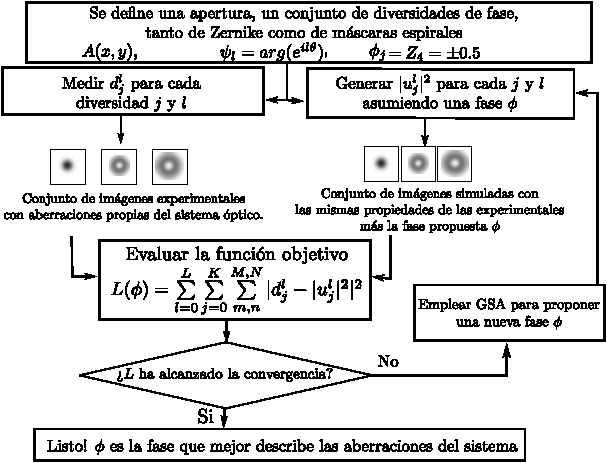
\includegraphics[width=\textwidth,keepaspectratio]{Caps/Imagenes/PDflux.pdf}
  \caption{Diagrama de flujo de PD coherente.}
  \label{fig:pdflux}
\end{figure}

En la Sección \ref{sec:generacion_vortices} se discutió que una de las formas más comunes de generar OVs es a través de SLMs, y cuando se emplean dichos elementos, si su modulación no es cercana a la ideal hay aberraciones inducidas en los OVs. Pero de acuerdo al planteamiento del algoritmo, $\phi$ representa todas las aberraciones del sistema y no es posible identificar de manera directa el aporte a las aberraciones provenientes de la baja modulación en fase del SLM y del sistema óptico, es decir, si bien $\phi$ describe las aberraciones del sistema, no da indicios de la fuente que las genera. Para discernir las aberraciones generadas por la baja modulación del SLM y el sistema óptico, se proponen entonces dos modificaciones sobre PD coherente mediante el empleo de las características reales del SLM.

\section{Modificaciones propuestas para diversidad de fase coherente}
\label{sec:pd12}

Tenemos un algoritmo basado en PD que se encarga de encontrar aberraciones presentes en OVs a partir de la comparación de los resultados experimentales con resultados ideales generados bajo las mismas características. Queremos distinguir las aberraciones causadas por la baja modulación del SLM y por el sistema óptico independientemente; para esto, se propone emplear la curva de modulación del SLM, es decir, analizar los efectos que tiene la modulación de fase real en la generación de OVs a través de simulaciones.\\

%Tenemos un algoritmo basado en PD que se encarga de encontrar aberraciones presentes en OVs a partir de la comparación de los resultados experimentales con resultados ideales generados bajo las mismas características. Queremos distinguir de dónde provienen las aberraciones, para esto, se propone emplear la curva de modulación real (CMR) del SLM, es decir, analizar los efectos que tiene la modulación en la generación de OVs a través de simulaciones

%Puesto que en PD hay una etapa de simulación de OVs, cuando se obtiene $u_j^l$, en esta se asume que la máscara espiral de fase es ideal, pero si tomamos la CMR del SLM entonces se encuentran que los OVs difieren de los ideales. Pensando en emplear la CMR, surge un nuevo simulador de OVs que se basa en los datos de modulación real. De esto nacen dos nuevas posibilidades para hacer PD, las cuales hemos denominado PD1 y PD2 y las trataremos a fondo a continuación. La Fig. \ref{fig:PD012} muestra las tres posibles maneras de generar OVs para PD. La primera de ellas proviene de una simulación ideal de los OVs, de esta se obtiene un conjunto de imágenes completamente ideales. La segunda consiste en la simulación de OVs que poseen una máscara de fase dada por la CMR y por tanto, si bien el sistema óptico es simulado, la modulación es real. La tercera son las imágenes aportadas por el sistema óptico. La pregunta es entonces, ¿qué información se puede obtener de la comparación de cada una de los diferentes generadores de OVs?

Puesto que en PD hay una etapa de simulación de OVs, cuando se obtiene $u_j^l$, en esta se asume que la máscara de fase espiral $\psi_l$ es ideal, de forma que al generar OVs a través de un sistema limitado por difracción, el resultado es un haz toroidal ideal. Pero como fue mostrado en la Sección \ref{sec:genvoslm}, si tomamos la curva de modulación del SLM y simulamos nuevamente la generación de OVs a través de un sistema limitado por difracción, el resultado es una aberración en los OVs a causa de la baja modulación. A partir del empleo de la modulación real del SLM en la simulación de los OVs se proponen dos modificaciones sobre PD coherente, de forma que a través de estas se puedan distinguirse las aberraciones causadas por la baja modulación en fase y las causadas por el sistema óptico. \\

Supongamos que las aberraciones recuperadas por PD coherente corresponden a $\phi_{coh}$, y que estas están compuestas de la aberración a causa de la modulación del SLM $\phi_{slm}$ y las contribuciones del sistema óptico $\phi_{so}$, de forma que,

\begin{equation}
\label{eqPDs}
\phi_{coh} = \phi_{so} + \phi_{slm},
\end{equation}

$\phi_{slm}$ está implícito en la modulación del SLM, entonces si podemos generar OVs que contengan información de la modulación real a través de un sistema limitado por difracción $o_j^l$, tendremos una nueva posibilidad como entrada para el algoritmo de PD coherente, como se muestra en la Fig. \ref{fig:PD012}. Allí se encuentran las tres posibles maneras de obtener OVs que sirven de entrada para PD coherente a partir de la fase que se quiera recuperar. La primera de ellas proviene de una simulación ideal de los OVs  $u_j^l$, en la cual se emplea un sistema limitado por difracción junto con una modulación ideal. La segunda consiste en emplear un sistema limitado por difracción que use la modulación real del SLM $o_j^l$, por tanto estas contienen la fase $\phi_{slm}$ que hace diferir los OVs del caso anterior. La tercera manera son los OVs producidos experimentalmente $d_j^l$.\\
%contienen la información no solo de la modulación del SLM, sino que además la de los elementos ópticos, de forma que podemos separar $\phi_{coh}$ en las contribuciones de la modulación  y del sistema óptico $\phi_{so}$, de forma que la aberración tiene la forma

%\begin{equation}
%\label{eqPDs}
%\phi_{coh} = \phi_{SO} + \phi_{SLM}
%\end{equation}
%si tomamos la CMR del SLM entonces se encuentran que los OVs difieren de los ideales. Pensando en emplear la CMR, surge un nuevo simulador de OVs que se basa en los datos de modulación real. De esto nacen dos nuevas posibilidades para hacer PD, las cuales hemos denominado PD1 y PD2 y las trataremos a fondo a continuación.

%Allí se encuentran las tres posibles maneras de obtener OVs que sirven de entrada para PD coherente a partir de la fase que se quiera recuperar. La primera de ellas proviene de una simulación ideal de los OVs, en la cual se emplea un sistema limitado por difracción junto con una  modulación ideal $u_j^l$, de esto se obtiene un conjunto de OVs ideales. La segunda consiste en emplear un sistema limitado por difracción que emplea la modulación real del SLM $o_j^l$, por tanto estas contienen la fase $\phi_{slm}$ que las hace diferir del caso anterior. La tercera manera son los OVs producidos experimentalmente $d_j^l$.




%La segunda consiste en la simulación de OVs que poseen una máscara de fase dada por la CMR y por tanto, si bien el sistema óptico es simulado, la modulación es real. La tercera son las imágenes aportadas por el sistema óptico. La pregunta es entonces, ¿qué información se puede obtener de la comparación de cada una de los diferentes generadores de OVs?

\begin{figure}[!ht]
  \centering
    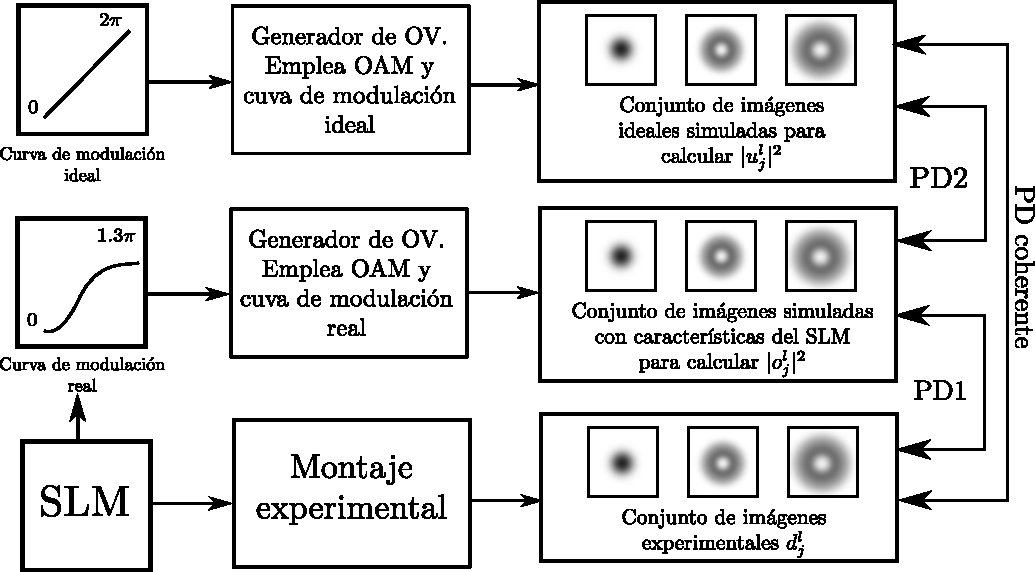
\includegraphics[width=\textwidth,keepaspectratio]{Caps/Imagenes/PD012fulx.pdf}
  \caption{Diagrama de las modificaciones sobre PD coherente.}
  \label{fig:PD012}
\end{figure}

Ahora, si en la Eq. \ref{eqPDs} consideramos que los OVs se producen en un sistema limitado por difracción con una modulación ideal, entonces $\phi_{so} = 0$ y $\phi_{slm} = 0$, por tanto, $\phi_{coh} = 0$, es decir, que si empleamos un sistema y una modulación ideal, no hay aberraciones. Si los OVs se generan con la modulación del SLM estos poseerán $\phi_{slm}$, como es el caso de $o_j^l$ y $d_j^l$, y debido a que ya se ha considerado la aberración por el SLM $\phi_{coh} = \phi_{so}$, y por ende si empleamos  en PD coherente, recuperaremos las aberraciones del sistema óptico $\phi_{so}$ independientes de la modulación del SLM, a esto le llamaremos PD1. Por último, si los OVs se generan por un sistema limitado por difracción y difieren únicamente por la modulación del SLM (empleando $u_{j}^{l}$ y $o_{j}^l$), $\phi_{so} = 0$ y $\phi_{coh} = \phi_{slm}$, a esto lo llamaremos PD2.\\

Como se muestra en la Fig. \ref{fig:PD012} si comparamos un conjunto de OVs generados idealmente con los que se generan desde el montaje experimental, estamos en el caso de PD coherente, es decir, un conjunto global de aberraciones $\phi_{coh}$ que presentan los OVs. Pero si la comparación es entre OVs ideales con aquellos generados por un sistema limitado por difracción con una modulación real (fila 2), la información que obtendremos corresponde a la aberración que introduce la modulación del SLM $\phi_{slm}$ (PD2). Esto es debido a que no estamos tomando resultados experimentales, de hecho, en ambos la propagación por el sistema óptico es simulada y se asume un sistema óptico limitado por difracción, lo que difiere es la característica de la modulación y por ende es de esperar que las aberraciones recuperadas correspondan a las inducidas únicamente por el SLM. Ahora si comparamos los resultados experimentales con los OVs que se generan mediante el sistema óptico limitado por difracción y la modulación del SLM, las aberraciones que se obtienen corresponden a las que son causadas por el sistema óptico $\phi_{so}$ (PD1). Esto es debido a que la aberración causada por la modulación del SLM se encuentra presente en ambos resultados y lo que difiere es el sistema óptico. La información obtenida con cada una de las modificaciones de PD se resume en la Tabla \ref{tab:pd012}.

\begin{center}
\begin{table}
	\centering
	\begin{tabular}{|c|p{8cm}|}
	\hline 
	PD coherente & Aberraciones globales 
	causadas por el SLM y el sistema óptico. \\ 
	\hline 
	PD1 & Aberraciones causadas por la 
	propagación de la luz a través del sistema óptico. \\ 
	\hline 
	PD2 & Aberraciones causadas por la 
	diferencia entre la modulación ideal-real. \\ 
	\hline 
	\end{tabular} 
	\caption{Información de las aberraciones recuperada de las modificaciones sobre PD coherente.}
	\label{tab:pd012}
\end{table}
\end{center}

Podemos definir dos nuevos funcionales similar a la Eq. \ref{eqDfuncCohere} para PD1 y PD2, puesto que solo modificamos las intensidades $|u_{j}^{l}|^2$, $|o_{j}^l|^2$ y $d_{j}^l$ de entrada para PD coherente, de forma que tendremos los siguientes funcionales,

\begin{equation}
	L_{PD1}(\phi) =\sum\limits_{l=0}^L \sum\limits_{j=0}^K \sum\limits_{u,v}^{M,N} |d_j^l(m,n) - |o_j^l(m,n,\phi)|^2|^2,
\end{equation}

\begin{equation}
	L_{PD2}(\phi) =\sum\limits_{l=0}^L \sum\limits_{j=0}^K \sum\limits_{u,v}^{M,N} \arrowvert |u_j^l(m,n)|^2 - |o_j^l(m,n,\phi)|^2 \arrowvert ^2.
\end{equation}


Los diferentes funcionales se resumen en uno genérico dado por,

\begin{equation}
\label{eqDfunc123}
 L(\phi) = \sum\limits_{l=0}^L \sum\limits_{j=0}^K \sum\limits_{u,v}^{M,N} |(d_j^l, |u_j^l|^2) - (|u_j^l|^2,|o_j^l|^2)|^2,
\end{equation}

aquí $(d_j^l, |u_j^l|^2)$ representa que según la modificación de PD se emplea $d_j^l$ ó $|u_j^l|^2$, al igual que $(|u_j^l|^2,|o_j^l|^2)$ determina si emplear $|u_j^l|^2$ ó $|o_j^l|^2$, las posibles combinaciones serán entonces: $d_j^l$ con $|u_j^l|^2$, que es el caso de PD coherente, $d_j^l$ con $|o_j^l|^2$, que es el caso de PD1 ó $|u_j^l|^2$ con $|o_j^l|^2$ que será el caso de PD2.\\

Por último, el esquema para el algoritmo de PD coherente modificado toma la forma presentada en la Fig. \ref{fig:pdfluxadd}. El proceso es similar al caso de PD coherente; primero se define una apertura $A(x,y)$ y un conjunto de aberraciones espirales y de aberraciones. A continuación se realizan las medidas experimentales de cada una de las diversidades y según la aberración que quiera recuperarse ($\phi _{coh}$, $\phi_{slm}$ ó $\phi_{so}$) se toma una de las simulaciones de los OVs producidos. Se evalúa la función objetivo y de acuerdo con el algoritmo de búsqueda de gradiente, se determina la aberración $\phi$ que hace tender $L$ a cero. Cuando se obtenga un valor de $L$ mínimo la fase $\phi$ recuperada corresponderá a la que se plantea con la versión de PD respectiva ($\phi _{coh}$, $\phi_{slm}$ ó $\phi_{so}$).
\begin{figure}[!ht]
  \centering
    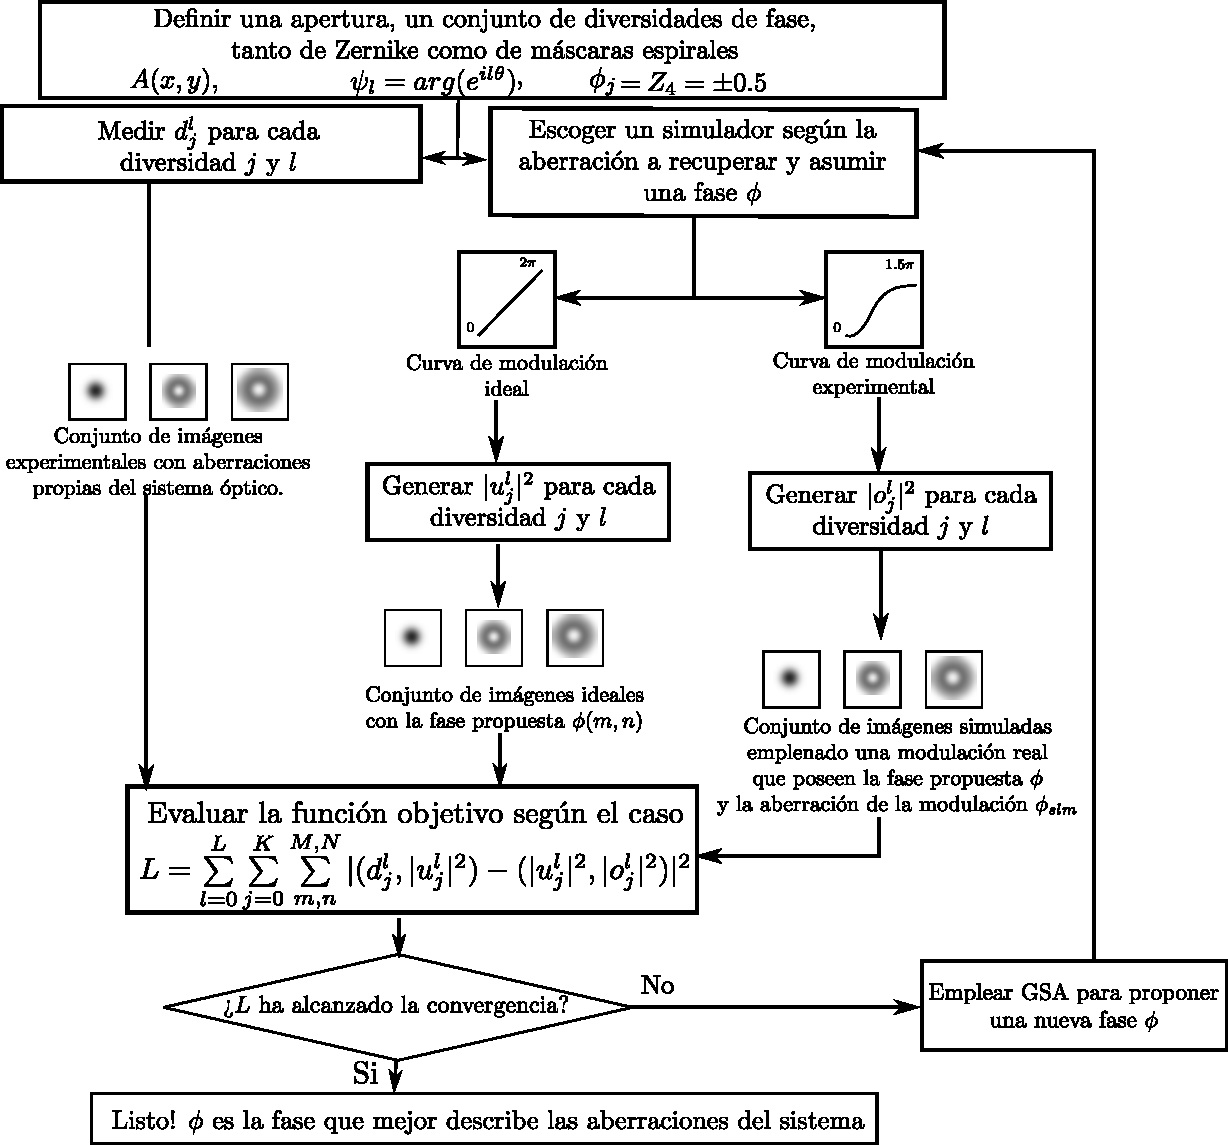
\includegraphics[width=\textwidth,keepaspectratio]{Caps/Imagenes/pdfluxadd.pdf}
  \caption{Diagrama de flujo de PD coherente con sus respectivas modificaciones.}
  \label{fig:pdfluxadd}
\end{figure}
